% !TEX root = ../paper.tex
\section{Discussion}
\label{sec:discussion}

When looking at the results on the effect of the four techniques, \pinch, \tilt, \swipe and \throw, as well as the two grid sizes, large and small, on the time per target, the results tell a rather interesting story. An overview of the results can be seen in \Cref{fig:timeResults}.

\begin{figure}[H]
	{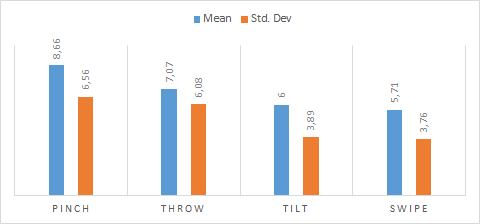
\includegraphics[width = 1\columnwidth ]{images/timeResults.png}} 
	\caption{
		Overview of the mean and standard deviation for each technique in regards to time per target.
	}
	\label{fig:timeResults}
\end{figure}

There was a significant difference between all techniques, with the exception of \swipe and \tilt. These were the two one handed techniques that were created. The range of movement needed in order to activate these two techniques was rather limited, the full motion could be achieved quite quickly and is quite similar for both of them.  This is why they are not statistically different from each other. \swipe and \tilt, are on average, at least a second faster then the other two. Their standard deviation are also smaller, which means that users were more consistent, with regards to how long it took to hit each target, with these two techniques. 

Looking at the two other techniques, \pinch and \throw, their times also reflect the range of motion needed in order to activate each technique. \pinch requires the user to pinch the shape on their phone, lift their hand up, direct it on the screen, and then finally let go. This can be seen in its mean, where it takes almost 1.59 seconds longer to perform than the second longest technique, \throw. \throw also requires a considerable range of motion in order to activate: point with one arm, select the shape on the phone with the other arm, bring your arm back and then finally swing it forward. Both two handed techniques take significantly longer time to perform than their one handed counter-parts.

\begin{figure}[H]
	{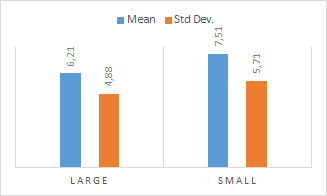
\includegraphics[width = 1\columnwidth ]{images/gridTimeResults.png}} 
	\caption{
		Overview of the mean and standard deviation for each grid size in regards to time per target.
	}
	\label{fig:gridtimeResults}
\end{figure}

\Cref{fig:gridtimeResults} shows an overview of the results of the effect of grid size on the time spent per target. We noticed that users would spent relatively little time getting into the general vicinity of the target, and would spend most of their time per attempt getting the pointer on top of the actual target. This would was more pronounced in the small grid, were users would perform smaller, more careful adjustments in order to not overshot the target, which can be seen in the small grid's mean time compared to the large grid.

\begin{figure}[H]
	{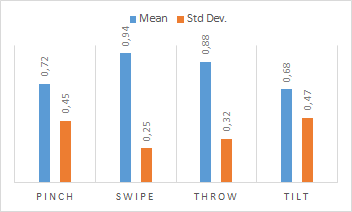
\includegraphics[width = 1\columnwidth ]{images/techHitResults.png}} 
	\caption{
		Overview of the mean and standard deviation for each technique in regards to hit rate per target.
	}
	\label{fig:gridhitResults}
\end{figure}

If we look at the results in regards to the effect of the technique on the hit ratio of each attempt, shown in \Cref{fig:gridhitResults}, it is interesting to note that the two techniques that were not significantly different from each other were \tilt and \pinch. These two techniques both used the hand that controlled the pointer to activate the technique. When tilting the phone forward, usually the hand would move together with the phone causing the pointer to displace itself from the users intended position. When releasing the \pinch, the Kinect would sometimes reevaluate the location of the hand joint, now that it could see the entire hand, which would cause the pointer to displace itself from the intended position. \pinch and \tilt were also the techniques that had the largest amount of activation errors due to the implementation of the system. Sometimes, users would show large amount of their palms to the Kinect during a \pinch, even though their hand was closed, causing the Kinect to evaluate that as an opening of the hand and activate the technique. \tilt would sometimes activate if the user moved the telephone around too quickly, especially when orienting the pointer up and down on the screen.  

\swipe and \throw both had reasonably   

\subsection{Limitations}

The intention with the \tilt technique was that the users would point and tilt with the phone, but because of our implementation, it was possible for users to point with one hand and tilt the phone with the other.
Again, because of our implementation of the \swipe technique, users were able to point with one hand and swipe with the other.